% =============================================================================
% Lecture 12: Bayesian Statistics III — Bayesian Linear Regression
% ECON 8310: Business Forecasting
% University of Nebraska at Omaha
% =============================================================================

\documentclass[aspectratio=169, 11pt]{beamer}

\input{header}

% ---- Lecture metadata --------------------------------------------------------
\title[Bayesian III: Regression]{Bayesian Statistics III: Bayesian Linear Regression}
\subtitle{ECON 8310: Business Forecasting --- Lecture 12}
\author{Department of Economics}
\institute{University of Nebraska at Omaha}

% =============================================================================
\begin{document}
% =============================================================================

\begin{frame}
  \titlepage
\end{frame}

% ---- Outline ----------------------------------------------------------------
\begin{frame}{Lecture Outline}
  \tableofcontents
\end{frame}

% =============================================================================
\section{Bayesian Linear Regression}
% =============================================================================

\sectionslide{Bayesian Linear Regression}{%
  The same regression you already know ---
  returning a distribution for every coefficient.}

% --- Slide: OLS vs Bayesian ---------------------------------------------------
\begin{frame}{OLS vs.\ Bayesian Regression: What Changes?}
  OLS, which you have fitted since Lecture 2, solves for one best coefficient vector:
  \[
    \hat{\boldsymbol{\beta}} = (\mathbf{X}^{\top}\mathbf{X})^{-1}\mathbf{X}^{\top}\mathbf{y}
  \]
  \vspace{-0.25cm}

  The Bayesian version uses Lecture 10's update rule instead:
  \[
    p(\boldsymbol{\beta} \mid \mathbf{y}) \;\propto\; p(\mathbf{y} \mid \boldsymbol{\beta}) \cdot p(\boldsymbol{\beta})
  \]
  \vspace{-0.25cm}

  \begin{keybox}
    \textbf{Every coefficient comes back as a distribution}: not an estimate plus an asymptotic
    error bar, but a full posterior you can ask questions of.
  \end{keybox}

  And Lecture 6 reappears: \textbf{regularization is a prior}. The posterior \emph{mode} under a
  Normal prior is the Ridge estimate; under a Laplace prior, it is the LASSO estimate.
\end{frame}

% --- Slide: PyMC ---------------------------------------------------------------
\begin{frame}{Bayesian Linear Regression in PyMC}
  \begin{examplebox}{Log units on log price, SNAP, events, series and trend}
    {\scriptsize\linespread{1.05}\selectfont
    \texttt{with pm.Model() as model:}\\
    \texttt{\mbox{}\ \ a\ \ \ \ \ \ \ = pm.Normal("a", y.mean(), 1, shape=J)\ \ \# one per series}\\
    \texttt{\mbox{}\ \ b\_price = pm.Normal("b\_price", 0, 1)\ \ \ \ \ \# weakly informative}\\
    \texttt{\mbox{}\ \ b\_snap\ \ = pm.Normal("b\_snap",\ 0, 1)}\\
    \texttt{\mbox{}\ \ b\_event = pm.Normal("b\_event", 0, 1)}\\
    \texttt{\mbox{}\ \ b\_trend = pm.Normal("b\_trend", 0, 1)}\\
    \texttt{\mbox{}\ \ sigma\ \ \ = pm.Exponential("sigma", 1.0)}\\
    \texttt{\mbox{}\ \ mu = a[idx] + b\_price*lpc + b\_snap*snap + b\_event*event + b\_trend*yr}\\
    \texttt{\mbox{}\ \ pm.Normal("obs", mu=mu, sigma=sigma, observed=y)}\\
    \texttt{\mbox{}\ \ idata = pm.sample(1000, tune=1500, chains=4)}\par
    }
  \end{examplebox}
  \textbf{Do not standardize log price} --- with both in logs \texttt{b\_price} is an
  \textbf{elasticity}, percent change in demand per percent change in price. \texttt{lpc} is log
  price centered within series, which fixed ESS 184 $\rightarrow$ 3{,}097.

\end{frame}

% =============================================================================
\section{Reading the Posterior}
% =============================================================================

\sectionslide{Reading the Posterior}{%
  Three questions you can ask a distribution
  that you cannot ask a point estimate.}

% --- Slide: reading a coefficient ------------------------------------------------
\begin{frame}{Reading a Posterior Coefficient}
  Fitted on the weekly panel, controlling for series and trend:
  \begin{center}
    {\small
    \begin{tabular}{lrrl}
      \toprule
      \textbf{Coefficient} & \textbf{Mean} & \textbf{94\% HDI} & \textbf{Reading} \\
      \midrule
      \texttt{b\_price} & $-0.493$ & $[-0.596,\ -0.387]$ & Inelastic: all of it above $-1$ \\
      \texttt{b\_trend} & $\phantom{-}0.110$ & $[\phantom{-}0.107,\ \phantom{-}0.113]$ & About 11\% growth per year \\
      \texttt{b\_snap} & $\phantom{-}0.036$ & $[\phantom{-}0.027,\ \phantom{-}0.046]$ & About a 3.7\% SNAP-week lift \\
      \texttt{b\_event} & $-0.003$ & $[-0.011,\ \phantom{-}0.004]$ & \textbf{Spans zero} \\
      \bottomrule
    \end{tabular}
    }
  \end{center}

  \vspace{-0.05cm}
  The \textbf{HDI} --- highest density interval --- is the shortest interval holding 94\% of the
  posterior, and it means what everyone wants: a 94\% probability the coefficient is inside.

  \vspace{0.15cm}
  \textbf{The last row is the useful one.} \texttt{b\_event}'s interval spans zero, so the data
  do not establish a direction. Two slides on, we ask whether it is also too small to matter.
\end{frame}

% --- Slide: probability questions ---------------------------------------------------
\begin{frame}{Asking the Posterior a Direct Question}
  \begin{examplebox}{Any question about $\beta$ is a count of samples: one line each}
    {\scriptsize\linespread{0.95}\selectfont
    \texttt{b = idata.posterior["b\_price"].values.ravel()}\\[-1pt]
    \texttt{(b < 0).mean()\ \ \ \ \ \# P(demand falls when price rises)}\\[-1pt]
    \texttt{(b < -1).mean()\ \ \ \ \# P(elastic: a price rise loses revenue)}\\[-1pt]
    \texttt{(b < -0.5).mean()\ \ \# P(a 1\% rise costs over 0.5\% of volume)}
    }
  \end{examplebox}
  \vspace{-0.1cm}
  {\centering
    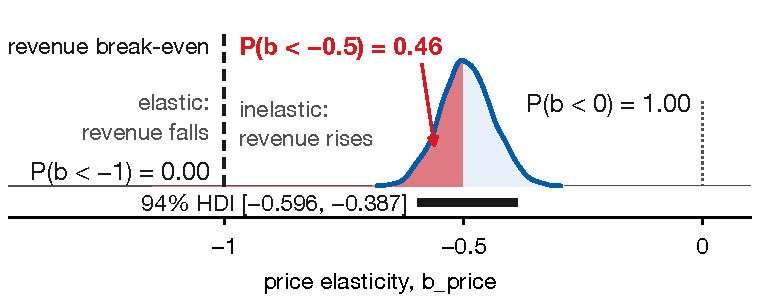
\includegraphics[height=3.2cm]{../Figures/Lecture12_BayesianRegression/posterior_area.pdf}\par}
  \vspace{-0.05cm}
  {\small Each answer is the share of the area past a line. Demand is \textbf{inelastic} in every
  draw; the half-percent question stays open. \textbf{A p-value gives only the direction.}}
\end{frame}

% --- Slide: ROPE -----------------------------------------------------------------------
\begin{frame}{Too Small to Matter? A ROPE}
  \texttt{b\_event}'s HDI spans zero: no direction. A \textbf{ROPE} --- region of practical
  equivalence --- asks a different question: is the effect too small to act on?
  \begin{center}
    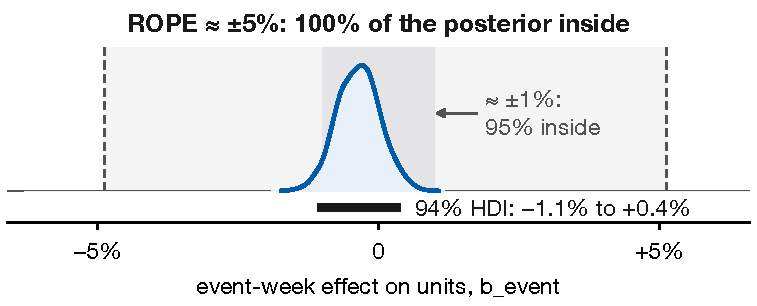
\includegraphics[height=3.15cm]{../Figures/Lecture12_BayesianRegression/rope_event.pdf}
  \end{center}
  \vspace{-0.3cm}
  {\small The width is a business choice, not a statistic. We use Homework 7's
  $|\beta| < 0.05$, about $\pm 5\%$ a week; even at $\pm 1\%$, 95\% is inside.}
  \begin{keybox}
    \small Spans zero and inside the ROPE: \textbf{negligible}, stop looking. Spans zero and wide:
    \textbf{still open}, get more data. ``Not significant'' cannot tell them apart.
  \end{keybox}
\end{frame}

% =============================================================================
\section{Causal Structure and DAGs}
% =============================================================================

\sectionslide{Causal Structure and DAGs}{%
  Which coefficients mean what you think they mean.}

% --- Slide: DAGs ----------------------------------------------------------------
\begin{frame}{Directed Acyclic Graphs}
  A \textbf{DAG} is a picture of what you believe causes what, drawn from domain knowledge
  \emph{before} the model. It decides which variables belong in the regression.

  \vspace{0.05cm}
  \begin{columns}[T]
    \begin{column}{0.57\textwidth}
      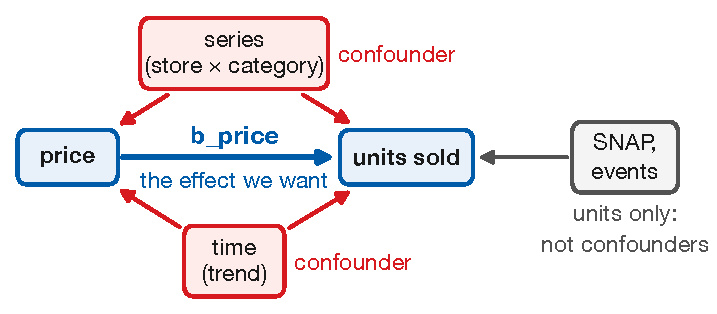
\includegraphics[width=\linewidth]{../Figures/Lecture12_BayesianRegression/dag.pdf}
    \end{column}
    \begin{column}{0.41\textwidth}
      {\small
      \key{Confounder}: causes both predictor and outcome. \textbf{Must} be controlled, or it
      leaks into your coefficient.

      \vspace{0.15cm}
      \textbf{Collider}: caused by both. Controlling for it \textbf{creates} a spurious
      association.\par}
    \end{column}
  \end{columns}

  \vspace{0.1cm}
  \textbf{So ``add every control you have'' is bad advice}, and no model fit settles it.

  \muted{\footnotesize\itshape Whether a DAG is right is a business question, not a statistical
  one.}
\end{frame}

% --- Slide: confounding measured --------------------------------------------------
\begin{frame}{Confounding, Measured}
  Two confounders move price and units together: the \textbf{category} and \textbf{time}.
  \begin{center}
    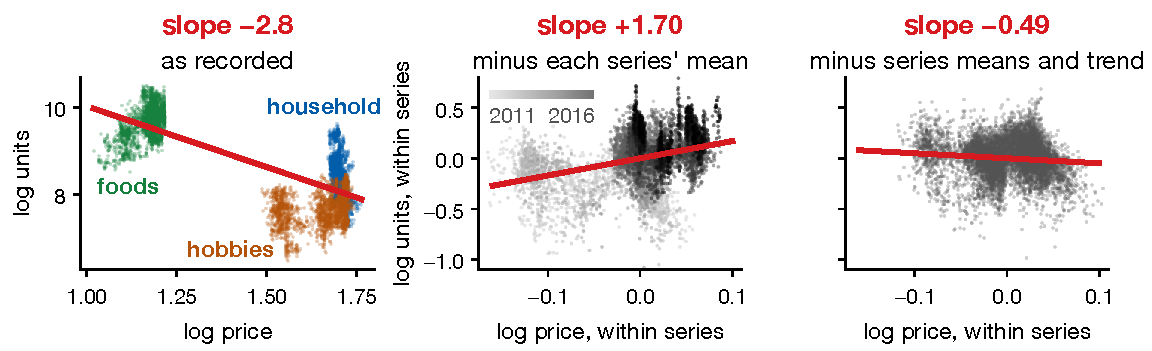
\includegraphics[height=3.62cm]{../Figures/Lecture12_BayesianRegression/confounding.pdf}
  \end{center}
  \vspace{-0.4cm}
  {\small Food is cheap and sells in volume; prices and volumes both rose, 2011--2016. Removing
  the series means alone flips the sign. With both removed: $-0.493$, HDI $[-0.596, -0.387]$. The
  naive $-2.805$, HDI $[-2.856, -2.756]$, is nearly six times too large, at half the width.}
  \begin{warningbox}
    \small Confidently, precisely wrong: a tight interval says the model is sure, not that it
    answers your question. Only the DAG protects you from an omitted confounder.
  \end{warningbox}
\end{frame}

% --- Slide: scenario analysis ------------------------------------------------------
\begin{frame}{Scenario Analysis with Posterior Samples}
  Push a scenario through the draws to get a \textbf{distribution of outcomes}, not one number.

  \begin{examplebox}{What if we raise price 5\%?}
    {\scriptsize\linespread{1.05}\selectfont
    \texttt{b = idata.posterior["b\_price"].values.ravel()}\\
    \texttt{pct\_change = 100 * (np.exp(b * np.log(1.05)) - 1)}\\[2pt]
    \texttt{pct\_change.mean(), np.percentile(pct\_change, [3, 97])}
    }
  \end{examplebox}

  With an elasticity near $-0.493$, a 5\% price rise implies roughly a \textbf{2.4\% fall in
  units}, 94\% of the posterior between $-2.9\%$ and $-1.9\%$.

  \vspace{0.1cm}
  \textbf{The decision follows.} Revenue changes by a factor $1.05^{\,1+b}$, which rises
  exactly when $b > -1$. Every draw is above $-1$, so $P(\text{revenue rises}) = 1.00$: about
  $+2.5\%$ on average.

  \muted{\footnotesize\itshape Valid only to the extent the DAG is --- this is a causal claim
  about intervening on price.}
\end{frame}

% =============================================================================
\section{Course Synthesis and Next Steps}
% =============================================================================

\sectionslide{Course Synthesis and Next Steps}{%
  From classical time series to Bayesian hierarchical models:
  a complete forecasting toolkit.}

% --- Slide: Method comparison ------------------------------------------------
\begin{frame}{Course Method Map}
  \begin{center}
    {\scriptsize
    \begin{tabular}{lllll}
      \toprule
      \textbf{Method} & \textbf{Data} & \textbf{Uncertainty} & \textbf{Interpretable} & \textbf{Strengths} \\
      \midrule
      ETS / ARIMA (L01--02) & Univariate TS & CI & High & Fast, automatic \\
      GAM / Prophet (L03) & TS + predictors & Limited & High & Nonlinear + interpretable \\
      Decision Tree (L04) & Tabular & No & High & Rule-based explanation \\
      Random Forest (L05) & Tabular & OOB error only & Medium & Robust, minimal tuning \\
      XGBoost (L05) & Tabular & No & Low & Interactions; 781 on our board \\
      Ridge / LASSO (L06) & Tabular & No & High & Best on our board: 744 \\
      FFN / 1D CNN (L07--08) & Tabular / TS & No & Low & Flexible nonlinear fits \\
      LSTM / Transformer (L09) & Sequences & No & Very low & Long-range dependencies \\
      Bayesian (L10--12) & Any & Full posterior & High & Uncertainty, small samples \\
      \bottomrule
    \end{tabular}
    }
  \end{center}
  \begin{keybox}
    \small No single method dominates. Choose based on:
    (1) data type and size, (2) need for uncertainty quantification,
    (3) need for interpretability, (4) time to deploy.
    In practice, combine: your scoreboard's winner for the point forecast (here, LASSO)
    and a Bayesian model for the intervals.
  \end{keybox}
\end{frame}

% --- Slide: Key takeaways ---------------------------------------------------
\begin{frame}{Lecture 12: Key Takeaways}
  \begin{keybox}
    {\small
    \begin{enumerate}
      \item \textbf{Bayesian regression}: a posterior per $\beta$, whose mode is Ridge (Normal)
            or LASSO (Laplace).
      \item \textbf{Ask the posterior directly}: mean, HDI, $P(\beta_j$ past a threshold$)$, mass in
            a ROPE.
      \item \textbf{Draw the DAG first}: control confounders (here, series \emph{and} time),
            never colliders.
      \item \textbf{Scenarios}: push a counterfactual through the draws to get a distribution of
            outcomes.
      \item \textbf{No single method is best}: pair an accurate point forecast with Bayesian
            intervals.
    \end{enumerate}
    }
  \end{keybox}
\end{frame}

% --- References ---------------------------------------------------------------
\begin{frame}[allowframebreaks]{References}
  \printbibliography[heading=none]
\end{frame}

% =============================================================================
\end{document}
% =============================================================================
